\chapter{Proofs and Experimental Results}\label{ResultsChapter}
The results of my research include proofs and experimental performance for the implementations described in Chapter \ref{MethodsChapter}. This chapter consists of two sections, one for generalization proofs and the other describing extraction and performance. Generalization proofs for the three Kernel Perceptron variants can be found in subsections \ref{KPProofs}, \ref{KPBProofs}, and \ref{KPDProofs}. The experiments run on the Kernel Perceptron variants were designed with three main questions in mind, including the difference between experimental and empirical generalization error, the generalization error and runtimes of the implementations on both real and synthetic datasets, and the difference in runtime between the Haskell implementations and unverified implementations in Python, the language most commonly used for machine learning research and applications. The extraction directives from Coq to Haskell for the three implementations are detailed in subsection \ref{DetailsHaskellExtraction}. Subsections \ref{SyntheticResults}, \ref{IrisResults}, \ref{SonarResults} describe the testing methodology for three datasets that were used to evaluate the experimental generalization error and analyze the runtime of training and testing each implementation. Finally, in subsection \ref{ResultsDiscussion}, the trends and results seen across datasets and implementations are outlined. The conclusions and future work for this research follow in Chapter \ref{ConclusionsChapter}.
\section{Generalization Proofs}\label{Proofs}
In the MLCert framework, much of the proof burden has been automated. For a new Learner representing a machine learning algorithm, there are two new lemmas that need to be proven. The first lemma proves the cardinality of the parameters used by the algorithm, which corresponds to the size of the parameter space. The second lemma applies the first in order to prove a generalization bound for the Learner as a whole. An example of the second lemma for a generic Learner is shown in Figure \ref{LearnerLemma}.

\begin{figure}
    \caption{Generalization Bound for a generic Learner}
    \label{LearnerLemma}
    \begin{lstlisting}
Lemma Learner_bound eps (eps_gt0 : 0 < eps) init : 
    @main A B Params Hypers Learner
      hypers m m_gt0 epochs d eps init (fun _ => 1) <=
    #|Params| * exp (-2%R * eps^2 * mR m).
    \end{lstlisting}
\end{figure}

The definition of main which is used in Figure \ref{LearnerLemma} can be found in the file ``learners.v''. Once main has been instantiated with the specifics of the Learner, such as its particular Params and Hypers, there are proofs in ``learners.v'' such as the lemma main\_bound which provide the machinery necessary to prove this inequality over the real numbers. As described by Bagnall and Stewart \cite{BS19}, MLCert uses Hoeffding's inequality, a type of Chernoff bound, to prove the generalization bound for a Learner. Most of the variables found in the Learner\_bound proof can be found in the Learner.t instantiation, but $\mathit{eps}$ is not part of the implementation. The value $\mathit{eps}$ is the difference between expected accuracy and empirical accuracy, which is usually a value between zero and one. The specific value of $\mathit{eps}$ is chosen to ensure that the resulting bound is nontrivial, as a bound greater than one is no longer useful for bounding generalization error. In the following subsections, the lemmas proving the generalization bounds for the Kernel Perceptron, Budget Kernel Perceptron, and Description Kernel Perceptron will be discussed.
\subsection{Kernel Perceptron Generalization Proofs}\label{KPProofs}
The bound for the Kernel Perceptron relies on the size of the parameter space. As proven in the lemma K\_card\_Params in the section KernelPerceptronGeneralization, the cardinality of the parameters for the Kernel Perceptron is shown in Equation \ref{KPParams}. This power of two is calculated by unfolding the definition of Params, which consists of the training set and a float array of size $m$. As all values are floating point numbers stored in 32 bits, the cardinality of a single floating point number is $2^{32}$. Therefore, as the dimensions of the training set are equal to $m$ training examples multiplied by $n$ dimensions, the cardinality of the training set is equal to $2^{m*n*32}$. The cardinality of a float array of size m is $2^{m * 32}$. 

\begin{equation} \label{KPParams}
 \#|Params| = 2^{(m*n*32 + m*32)}
\end{equation}

Kcard\_Params is central to the proof of the generalization bounds of the Kernel Perceptron in the lemma KPerceptron\_bound, which is defined in Figure \ref{KPLemma}. The generalization bound for the Kernel Perceptron is very loose, as growth in the size of the training set causes exponential growth in the generalization error. This limits the usefulness of the Kernel Perceptron's generalization bound, as a loose generalization bound provides few guarantees of performance or correctness. However, the Kernel Perceptron bound serves as a baseline for the generalization bounds of the Budget Kernel Perceptron and the Description Kernel Perceptron.

\begin{figure}
    \caption{Generalization Bound for the Kernel Perceptron}
    \label{KPLemma}
    \begin{lstlisting}
Lemma Kperceptron_bound eps (eps_gt0 : 0 < eps) init : 
    @main A B Params KernelPerceptron.Hypers 
      (@KernelPerceptron.Learner n m KPsupport_vectors H K)
      hypers m m_gt0 epochs d eps init (fun _ => 1) <=
    2^(m*n*32 + m*32) * exp (-2%R * eps^2 * mR m).
    \end{lstlisting}
\end{figure}

\subsection{Budget Kernel Perceptron Generalization Proofs}\label{KPBProofs}
The Budget Kernel Perceptron has a similar bound on the cardinality of the parameter space. However, the parameter space for the Budget Kernel Perceptron is not dependent on $m$, the size of the training set, whatsoever. Instead, the parameter space relies on the size of the support set. In code and proofs, the size of the support set is listed as $(S sv)$, which is equivalent to $sv + 1$. The successor of $sv$ is used so that the budget update procedure is always possible regardless of the value of $sv$, as there will be at least one support vector able to be replaced.
\\Like the Kernel Perceptron, the Budget Kernel Perceptron stores the support set and a float array. The float array is of size $(S sv)$, so its cardinality is $2^{32 * (S sv)}$. The support set stores $(S sv)$ training examples, which consist of one float value for each of the $n$ dimensions of the data, plus a Boolean value for the label of the support vector. Therefore, the cardinality of each training example in the support set is $2^{1 + n * 32}$. The full cardinality of the Budget Kernel Perceptron Params is given in Equation \ref{KPBParams}. The lemma proving this bound is found in the section KernelPerceptronGeneralizationBudget, named Kcard\_Params\_Budget.

\begin{equation} \label{KPBParams}
 \#|Params| = 2^{((32*(S sv) + ((1 + n * 32)*(S sv))))}
\end{equation}

Figure \ref{KPBLemma} shows the lemma for the generalization bound of the Budget Kernel Perceptron, which uses Kcard\_Params\_Budget in its proof. The INR term before the cardinality of the parameter set is an injection from the encoding of natural numbers to the real numbers as part of the proof of this bound. Comparing the bound of the Budget Kernel Perceptron to the Kernel Perceptron, the overall structure of the two bounds is similar when the number of training examples is the same. However, because the support set can be significantly smaller than the number of training examples, the Budget Kernel Perceptron's bound grows much less slowly than that of the base Kernel Perceptron. 

\begin{figure}
    \caption{Generalization Bound for the Budget Kernel Perceptron}
    \label{KPBLemma}
    \begin{lstlisting}
Lemma Kperceptron_bound_budget eps (eps_gt0 : 0 < eps) init : 
    @main A B Params KernelPerceptronBudget.Hypers 
      (@KernelPerceptronBudget.Learner n sv F K U)
      hypers m m_gt0 epochs d eps init (fun _ => 1) <=
    INR 2^((32*(S sv) + ((1 + n * 32)*(S sv)))) * exp (-2%R * eps^2 * mR m).
    \end{lstlisting}
\end{figure}

\subsection{Description Kernel Perceptron Generalization Proofs}\label{KPDProofs}

The generalization bound for the Description Kernel Perceptron is similar to that of the Budget Kernel Perceptron. First, we must define the cardinality of the parameter space used by the Description Kernel Perceptron. The parameters store a single float32 value paired with $(S des)$ support vectors. The successor of $des$ is used as the size of the support set, so that support vector replacement is always possible. Like with the Budget Kernel Perceptron, the cardinality of each support vector in the support set is $2^{1 + n * 32}$, which stores a single Boolean label as well as $n$ float32 values. However, because there is not a float value for every support vector, only the cardinality of a single float32 must be added to the cardinality of the entire support set. The cardinality of the Description parameters is shown in Equation \ref{KPDParams}.

\begin{equation} \label{KPDParams}
 \#|Params| = 2^{((32 + ((1 + n * 32)*(S des))))}
\end{equation}

Figure \ref{KPDLemma} shows the generalization bound of the Description Kernel Perceptron in the lemma Kperceptron\_bound\_Des. This bound is similar to the bound of the Budget Kernel Perceptron, but is tighter because there is only one float32 value instead of a float32 value per support vector. This small difference means that if the budget is the same as the number of mistakes for a specific dataset, the Description Kernel Perceptron will have a lower bound. 

\begin{figure}
    \caption{Generalization Bound for the Description Kernel Perceptron}
    \label{KPDLemma}
    \begin{lstlisting}
Lemma Kperceptron_bound_Des eps (eps_gt0 : 0 < eps) init : 
    @main A B Params KernelPerceptronDes.Hypers 
      (@KernelPerceptronDes.Learner n des F K)
      hypers m m_gt0 epochs d eps init (fun _ => 1) <=
    INR 2 ^ (32 + (1 + n * 32) * (S des)) * exp (-2%R * eps^2 * mR m).
    \end{lstlisting}
\end{figure}

\section{Haskell Extraction and Performance Experiments}\label{HaskellExtractionPerformance}
In order for the Coq implementations to be run, these implementations must be extracted to Haskell. The file ``extraction\_hs.v'' contains extraction directives for Haskell so that some Coq functions and data structures are extracted properly. The last Coq module for each implementation uses the extractible\_main definition, found in ``learners.v'', to also provide the necessary machinery that Learner.t relies on. The extracted Coq code is written to two sets of Haskell files located in the directory hs/KernelPerceptron/ in MLCert.
\\The extracted Haskell code for a machine learning algorithm does not contain code to initialize the system with training and testing data or functions to display accuracy and generalization error results to the user. Unverified Haskell drivers have been written for these implementations, which include the extracted Haskell code as a module. The Haskell drivers for the Kernel Perceptron implementations can also be found in the hs/KernelPerceptron/ directory.
\subsection{Details of Haskell Extraction}\label{DetailsHaskellExtraction}
The extraction directives for the Kernel Perceptron can be found in the section KPerceptronExtraction in the file ``kernelperceptron.v''. This section extracts the Kernel Perceptron to the Haskell file ``KPerceptron.hs'', a Haskell module that can be included by a Haskell driver program. This file is extracted to the two locations in MLCert where Haskell driver programs reside: hs/KernelPerceptron/ and hs/KernelPerceptron/timing\_drivers/. The Budget Kernel Perceptron and Description Kernel Perceptron each have their own extraction directives to extract ``KPerceptronBudget.hs'' and ``KPerceptronDes.hs'' to these same locations. 
\\There are four different kinds of Haskell driver programs for a variety of different purposes. All driver programs report the training accuracy, test accuracy, and generalization error for the dataset run by that driver. Several also print the model produced by training. The drivers are differentiated by their file names, which identify the purpose of the drivers.
\\``KPerceptronXOR.hs'' tests that the Kernel Perceptron using a quadratic kernel can classify the XOR function with 100\% accuracy. The linear kernel cannot be used because the XOR function is not linearly separable. The four samples for this function are specified in the driver, along with the quadratic kernel for the prediction function. When run, this driver demonstrates that the Kernel Perceptron behaves as expected with the quadratic kernel and is able to classify data that is not linearly separable. This is the only driver that uses nonlinear data and a nonlinear kernel function for prediction.
\\Each implementation has a driver that generates a new linearly separable dataset using a random number generator to test that the implementation can execute. These drivers have Test in their file names and first randomly generating $n$ floating point values between negative one and one to determine a linear hyperplane. Training and testing examples are generated by this method and classified using the hyperplane, creating a synthetic dataset that is linearly separable by construction. These synthetic datasets test that the implementations have been set up correctly and can classify linear data. However, because the datasets are generated differently for each run of the program, these drivers cannot be used to compare implementations.
\\To compare the accuracy of an implementation on a specific dataset, each implementation has a driver which reads a dataset from files and performs training and testing. These drivers have RunFile in their file names. The drivers require that the input dataset be stored in two files, one containing the training set and the other containing the test set. The dataset files must also be formatted with one example per line and values separated by commas. The first value of the line must be a positive unique integer, which is used by the Kernel Perceptron to differentiate between the training examples for updates. The last value must be either True or False, corresponding to the label for the example. As long as the dataset files are formatted correctly, the driver will train and test on this dataset and report the accuracy and generalization error for this dataset. Only one dataset is run by this driver.
\\Finally, to time the execution of training and testing on a dataset, drivers with FileIO in their name read in one or more datasets. The FileIO drivers run training and testing five times and report the time in seconds. Each implementation has a FileIO driver which can run multiple datasets with varying dimensions. The drivers do not time reading the dataset files and use the same data format as the RunFile drivers. 
\\In the following subsections, I will detail my testing methodology on three datasets, two real datasets downloaded from the UCI Machine Learning Repository \cite{DG17} and a synthetic dataset created from randomly generated linear hyperplanes. The Iris Data Set \cite{Fis36} and Sonar Mines vs. Rocks Data Set \cite{SG88} were formatted to be more easily read into the driver programs. Each of the following subsections describes the dataset under test, the experimental setup and drivers used, the calculated generalization error, and the timing results for training and testing.
\subsection{Synthetic Dataset Performance Results}\label{SyntheticResults}
A synthetic dataset was created specifically to test the performance of the Kernel Perceptron and its variants. There are 20 independent trials in this dataset with training and testing sets based on randomly generated data separated by a randomly oriented linear hyperplane. Each trial contains 1000 training examples and 1000 test examples, each with three dimensions. These datasets were created by recording and formatting the output of 20 runs of ``KPerceptronTest.hs''. 
\\Because the Kernel Perceptron variants are all deterministic, the generalization error results were found using the RunFile driver for each implementation. All implementations ran for five epochs. The Budget Kernel Perceptron limited the size of the support set to 100 examples, 10\% of the training set, and the Description Kernel Perceptron was similarly limited to 100 mistakes. 
\\The generalization error of the three implementations is graphed in Figure \ref{SyntheticGenErrFig}. The Kernel Perceptron and Budget Kernel Perceptron have the same training and testing error for all 20 synthetic trials, while the Description Kernel Perceptron tends to have slightly worse training and testing accuracy and increased generalization error on some trials. The greatest observed generalization error is 1.4\% for the Description Kernel Perceptron in Trial 8.

\begin{figure}[p]
 \caption{Synthetic Generalization Error}
 \label{SyntheticGenErrFig}
 \begin{center}
  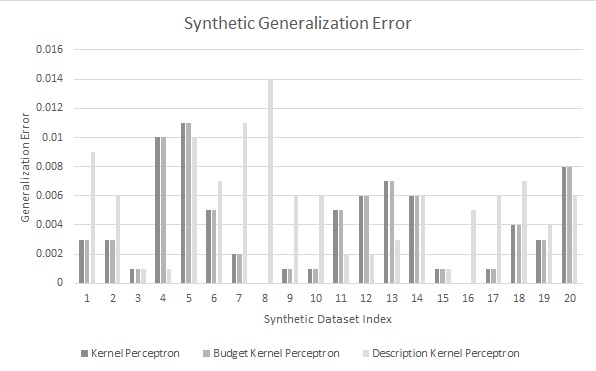
\includegraphics[scale=0.7]{SyntheticGenErr}
 \end{center}
\end{figure}

Table \ref{tab:avesyntheticaccgen} provides statistics across the synthetic trials for average training and testing accuracy and generalization error, along with the 95\% confidence interval for each implementation. Because the Kernel Perceptron and Budget Kernel Perceptron had the same performance across all trials, their averages and confidence interval are the same. The Description Kernel Perceptron's averages reflect its tendency to have lower accuracy and increased generalization error, and its confidence interval is larger than the other two implementations. For many of these trials, the Description Kernel Perceptron would require several more mistakes to have the same performance as the Kernel Perceptron and Budget Kernel Perceptron.

\begin{table}[p]
 \begin{center}
  \caption{Average Synthetic Generalization Error and Confidence Intervals}
  \label{tab:avesyntheticaccgen}
  \begin{tabular}{l|c|c|c}
  \textbf{ } & \textbf{KP} & \textbf{Budget KP} & \textbf{Description KP}\\
  \hline
  \textbf{Average Training Accuracy} & 98.61\% & 98.61\% & 96.915\%\\
  \textbf{Average Testing Accuracy} & 98.58\% & 98.58\% & 96.87\%\\
  \textbf{Average Generalization Error} & 0.39\% & 0.39\% & 0.565\%\\
  \textbf{95\% Confidence Interval} & 0.001435352 & 0.001435352 & 0.001539834\\
  \end{tabular}
 \end{center}
\end{table}

Using the generalization bounds as proven in Section \ref{Proofs}, the number of training examples, dimensionality of the data, and size of the support set can be input to determine if the observed generalization error compares to the calculated bound. Table \ref{tab:syntheticgencalc} shows the generalization bound for the two extreme values of $\mathit{eps}$, which are greater than zero and less than or equal to one. Unfortunately, for both of these values, all the implementations have vacuous bounds far greater than one. With the settings used in the above experiments, the calculated generalization bounds are unable to be compared to the observed generalization error. 

\begin{table}[p]
 \begin{center}
  \caption{Synthetic Generalization Bound Calculations}
  \label{tab:syntheticgencalc}
  \begin{tabular}{l|c|c|c}
  \textbf{ } & \textbf{KP} & \textbf{Budget KP} & \textbf{Description KP}\\
  \hline
  \textbf{Training Examples} & 1000 & 1000 & 1000\\
  \textbf{Dimensionality} & 3 & 3 & 3\\
  \textbf{Support Vectors} & 1000 & 100 & 100\\
  \textbf{eps = 0.001} & 6.89567E+38531 & 1.93230E+3883 & 4.19807E+2929\\
  \textbf{eps = 1} & 1.78025E+37663 & 4.98862E+3014 & 1.08381E+2061\\
  \end{tabular}
 \end{center}
\end{table}

Worse still is the fact that the Kernel Perceptron always produces vacuous bounds. Because all training examples are support vectors, the smallest possible training set is a single example. The smallest possible dimensionality of data is one dimensional. Therefore, the generalization bound for the smallest possible dataset of a single one-dimensional training example stored as a float32 value is shown in Equation \ref{KPBoundBad}. This bound is calculated to be 1.84467E+19 for $\mathit{eps}$ = 0.001 and 2.49650E+18 for $\mathit{eps}$ = 1. The bound becomes even more vacuous as the dimensionality of the data and number of examples increases. Because of this, the Kernel Perceptron cannot be used to compare calculated generalization error to generalization error observed in experiments.

\begin{equation} \label{KPBoundBad}
 2^{(m*n*32 + m*32)} * e^{-2*eps^{2}*m} = 2^{(1*1*32 + 1*32)} * e^{-2*eps^{2}*1} = 2^{64}*e^{-2eps^{2}}
\end{equation}

To determine if the Budget Kernel Perceptron and Description Kernel Perceptron produce nonvacuous bounds, different support set sizes and values of eps were input into their generalization bounds. With the settings listed in Table \ref{tab:syntheticlimitedgen}, nonvacuous bounds were found for both variants. The synthetic dataset was used to evaluate the effect of a limited budget for the Budget Kernel Perceptron and a limited number of mistakes for the Description Kernel Perceptron. Both implementations have a generalization bound of about 9\% for a three-dimensional dataset containing one thousand training examples and two support vectors or mistakes for Budget and Description, respectively. To produce these values, $\mathit{eps}$ must be set to 0.301 for the Budget Kernel Perceptron and 0.282 for the Description Kernel Perceptron. The generalization error produced by these implementations with limited budget and mistakes is graphed in Figure \ref{SyntheticGenErr2Fig}. Overall, the training and testing accuracy for both implementations is far lower than the accuracy produced with larger support sets, but the difference between training and testing accuracy remains small. The greatest observed generalization error observed for the Budget Kernel Perceptron is 5.7\% and for the Description Kernel Perceptron is 4.8\%, well below the 9\% calculated bound, which validates the theoretical bound proven in Coq for these implementations.

\begin{figure}[p]
 \caption{Synthetic Generalization Error using Limited Budget and Mistakes}
 \label{SyntheticGenErr2Fig}
 \begin{center}
  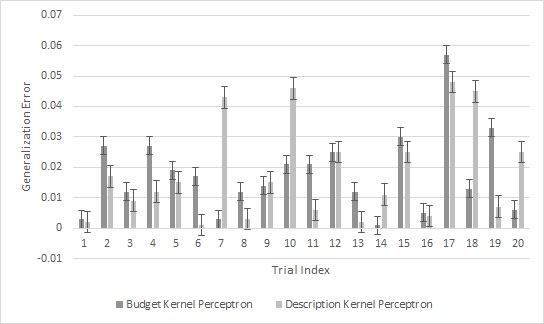
\includegraphics[scale=0.9]{SyntheticGenLimit} 
 \end{center}
\end{figure}

\begin{table}[p]
 \begin{center}
  \caption{Synthetic Generalization Error and Confidence Intervals using Limited Budget and Mistakes}
  \label{tab:syntheticlimitedgen}
  \begin{tabular}{l|c|c}
  \textbf{ } & \textbf{Budget KP} & \textbf{Description KP}\\
  \hline
  \textbf{Training Examples} & 1000 & 1000\\
  \textbf{Dimensionality} & 3 & 3\\
  \textbf{Support Vectors} & 2 & 2\\
  \textbf{eps} & 0.301 & 0.282\\
  \hline
  \textbf{Calculated Bound} & 9.35\% & 9.10\%\\
  \textbf{Greatest Observed Generalization Error} & 5.7\% & 4.8\%\\
  \hline
  \textbf{Average Training Accuracy} & 76.89\% & 78.625\%\\
  \textbf{Average Testing Accuracy} & 76.6\% & 78.11\%\\
  \textbf{Average Generalization Error} & 1.79\% & 1.805\%\\
  \textbf{95\% Confidence Interval} & 0.005794861 & 0.007007097\\
  \end{tabular}
 \end{center}
\end{table}

The runtimes of the three implmentations were also evaluated to compare training and testing performance. The runtime for each trial was tested five times to determine average training and testing. Figure \ref{SyntheticKernelTiming} shows the synthetic timing results for the Kernel Perceptron. All runtimes were around 200 seconds, with little variation between trials. The averages for each trial and their 95\% confidence intervals are listed in Table \ref{tab:synthetictiming}.

\begin{figure}[p]
 \caption{Kernel Perceptron Synthetic Timing}
 \label{SyntheticKernelTiming}
 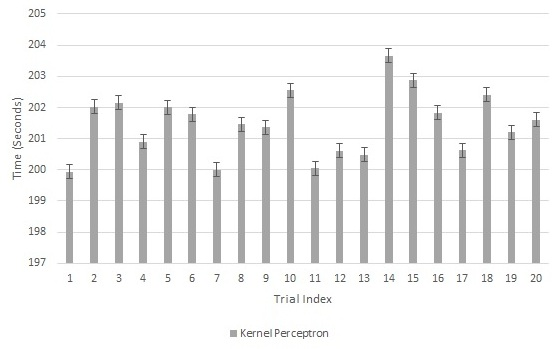
\includegraphics[scale=0.7]{KernelSyntheticTiming}
\end{figure}

The Budget Kernel Perceptron and Description Kernel Perceptron execute much faster than the Kernel Perceptron because their models are significantly smaller. Figure \ref{SyntheticBudgetDesTiming} shows the synthetic timing results for these two implementaitons. The Budget Kernel Perceptron took around 0.35 seconds to train and test, while the Description Kernel Perceptron took around 0.29 seconds. The Description Kernel Perceptron has the smallest model of the three implementations, causing it to have the fastest runtime. Table \ref{tab:synthetictiming} shows the averages and confidence intervals for each trial.

\begin{figure}[p]
 \caption{Budget and Description Kernel Perceptron Synthetic Timing}
 \label{SyntheticBudgetDesTiming}
 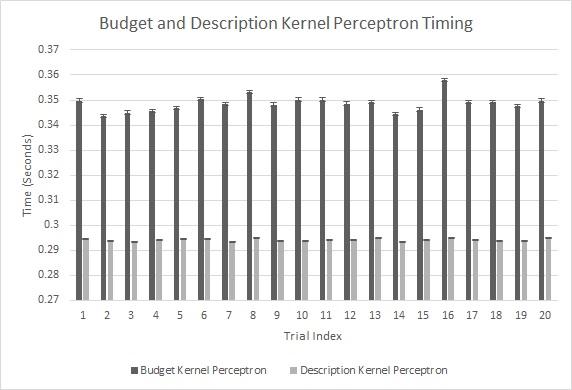
\includegraphics[scale=0.7]{BudgetDesSyntheticTiming}
\end{figure}

The confidence intervals for the Kernel Perceptron trials are much larger than the Budget and Description Kernel Perceptron trials because the runtimes for the Kernel Perceptron vary by seconds, as opposed to hundredths of seconds for the Budget and Description Kernel Perceptrons. These runtimes show that it is possible for the Budget and Description Kernel Perceptrons to have the same or similar accuracy as the Kernel Perceptron while training and testing in a shorter amount of time. 

\begin{table}[p]
 \begin{center}
  \caption{Synthetic Average Runtimes (Seconds) and Confidence Intervals}
  \label{tab:synthetictiming}
  \begin{tabular}{l|c|c|c|c|c|c}
  \textbf{Trial} & \textbf{KP} & \textbf{95\% CI} & \textbf{Budget KP} & \textbf{95\% CI} & \textbf{Description KP} & \textbf{95\% CI}\\
  \hline
  \textbf{1} & 199.943 & 3.17258 & 0.3498 & 0.05499 & 0.2946 & 0.05606\\
  \textbf{2} & 202.025 & 2.44561 & 0.3436 & 0.05116 & 0.2938 & 0.05499\\
  \textbf{3} & 202.145 & 2.78125 & 0.345 & 0.05245 & 0.2932 & 0.05529\\
  \textbf{4} & 200.901 & 2.62953 & 0.3456 & 0.05263 & 0.294 & 0.05441\\
  \textbf{5} & 202.012 & 2.97056 & 0.3468 & 0.05351 & 0.2946 & 0.05557\\
  \textbf{6} & 201.786 & 2.46189 & 0.3504 & 0.05567 & 0.2944 & 0.05666\\
  \textbf{7} & 199.996 & 2.66681 & 0.3484 & 0.05175 & 0.2934 & 0.05422\\
  \textbf{8} & 201.455 & 3.07707 & 0.3532 & 0.05527 & 0.295 & 0.05440\\
  \textbf{9} & 201.362 & 2.92524 & 0.3482 & 0.05479 & 0.2936 & 0.05558\\
  \textbf{10} & 202.546 & 2.92950 & 0.3502 & 0.05332 & 0.2938 & 0.05452\\
  \textbf{11} & 200.051 & 2.58570 & 0.3502 & 0.05332 & 0.2942 & 0.05432\\
  \textbf{12} & 200.609 & 3.10256 & 0.3486 & 0.05215 & 0.294 & 0.05537\\
  \textbf{13} & 200.479 & 3.28990 & 0.3492 & 0.05331 & 0.2948 & 0.05647\\
  \textbf{14} & 203.655 & 3.41870 & 0.3444 & 0.05226 & 0.2934 & 0.05323\\
  \textbf{15} & 202.866 & 4.18980 & 0.3462 & 0.05384 & 0.294 & 0.05489\\
  \textbf{16} & 201.827 & 3.75820 & 0.358 & 0.05232 & 0.295 & 0.05587\\
  \textbf{17} & 200.627 & 3.80374 & 0.3492 & 0.05333 & 0.2942 & 0.05528\\
  \textbf{18} & 202.409 & 3.09442 & 0.3492 & 0.05381 & 0.2938 & 0.05450\\
  \textbf{19} & 201.203 & 2.51938 & 0.3476 & 0.05410 & 0.2938 & 0.05646\\
  \textbf{20} & 201.605 & 2.93406 & 0.3498 & 0.05351 & 0.295 & 0.05442\\
  \end{tabular}
 \end{center}
\end{table}

The timing analysis of the Kernel Perceptron variants on the same datasets demonstrates how the runtimes for training and testing compare against implementations in the same language. However, because Haskell is not commonly used for machine learning tasks, the previous timing results do not indicate how the Haskell implementations compare against implementations in another language. Python is currently one of the languages of choice for machine learning research and applications because of libraries such as Numpy and Scipy that optimize scientific computing and machine learning algorithms. To compare the performance of Haskell to Python, the Budget Kernel Perceptron was chosen to be implemented in Python because it tends to have higher accuracy than the Description Kernel Perceptron with less required resources than the Kernel Perceptron. 
\\Two unverified Python scripts were written to be run on synthetic data. The first script, ``BudgetPython.py'', is close to a direct translation of the Haskell implementation into Python without modifications to improve performance in Python. This script will be referred to as the naive Python implementation. Many of the function and variable names were kept the same and the overall data structures and steps are the same. However, several changes were necessary. For example, the Haskell implementation uses 32-bit floating point values, but the naive Python implementation uses the built-in float type, which is 64-bit. Instead of recursion or folds, the naive Python implementation uses for loops to iterate through the parameters or the training and testing sets. Finally, the Python scripts do not use global variables, which are used in the Haskell driver files to specify the size and shape of the training set, so that multiple shapes and sizes of data sets can be run by the same functions. These changes simplify the Budget Kernel Perceptron implementation while not changing many of the underlying functions and data structures.
\\The second script, ``BudgetPythonNumpy.py'', improves on the naive Python implementation by using Numpy data structures and functions. Several types were modified to be more compatible with Numpy, such as the type of parameters. Instead of a list of tuples, where each tuple contains the float32 value, data, and label for a support vector, the Numpy Python implementation uses a tuple containing three Numpy arrays, so that the float32 values, data, and labels are in separate arrays. This change to the structure of the parameters makes vectorization much easier and facilitated the use of Numpy functions for computation. The Numpy Python and naive Python implementations produce the same results for accuracy and generalization error, but through calculations with different structures.
\\For both scripts, the timing procedure in Python was the same as in Haskell. For each trial of the synthetic dataset, the file input to read and format the dataset was not timed, but training and testing were timed five times to average the results. For each trial, the training and testing accuracy was compared to the Haskell implementation to ensure that all three Budget Kernel Perceptron implementations produced the same generalization error.

\begin{figure}[p]
 \caption{Python and Haskell Budget Kernel Perceptron Synthetic Timing}
 \label{SyntheticPythonHaskellTiming}
 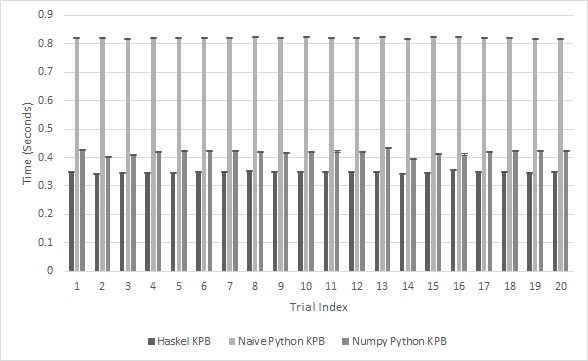
\includegraphics[scale=0.9]{PythonSyntheticTiming}
\end{figure}

\begin{table}[p]
 \begin{center}
  \caption{Python Budget Kernel Perceptron Runtimes and Confidence Intervals}
  \label{tab:pythontiming}
  \begin{tabular}{l|c|c|c|c|c|c}
  \textbf{Trial} & \textbf{Budget} & \textbf{95\% CI} & \textbf{Naive} & \textbf{95\% CI} & \textbf{Numpy} & \textbf{95\% CI}\\
  \textbf{} & \textbf{Haskell} & \textbf{} & \textbf{Python} & \textbf{} & \textbf{Python}\\
  \hline
  \textbf{1} & 0.3498 & 0.05499 & 0.82 & 0.00139 & 0.4266 & 0.00380\\
  \textbf{2} & 0.3436 & 0.05116 & 0.8216 & 0.00220 & 0.4024 & 0.00078\\
  \textbf{3} & 0.345 & 0.05245 & 0.819 & 0.00107 & 0.4088 & 0.00073\\
  \textbf{4} & 0.3456 & 0.05263 & 0.8198 & 0.00169 & 0.4208 & 0.00073\\
  \textbf{5} & 0.3468 & 0.05351 & 0.8216 & 0.00274 & 0.4236 & 0.00048\\
  \textbf{6} & 0.3504 & 0.05567 & 0.822 & 0.00107 & 0.4218 & 0.00073\\
  \textbf{7} & 0.3484 & 0.05175 & 0.8206 & 0.00118 & 0.4218 & 0.00114\\
  \textbf{8} & 0.3532 & 0.05527 & 0.8248 & 0.00209 & 0.4192 & 0.00243\\
  \textbf{9} & 0.3482 & 0.05479 & 0.82 & 0.00107 & 0.4146 & 0.00078\\
  \textbf{10} & 0.3502 & 0.05332 & 0.8232 & 0.00157 & 0.4184 & 0.00048\\
  \textbf{11} & 0.3502 & 0.05332 & 0.822 & 0.00196 & 0.421 & 0.00062\\
  \textbf{12} & 0.3486 & 0.05215 & 0.8206 & 0.00147 & 0.4188 & 0.00114\\
  \textbf{13} & 0.3492 & 0.05331 & 0.8232 & 0.00293 & 0.4326 & 0.00048\\
  \textbf{14} & 0.3444 & 0.05226 & 0.819 & 0.00164 & 0.396 & 0.00206\\
  \textbf{15} & 0.3462 & 0.05384 & 0.8234 & 0.00202 & 0.4136 & 0.00078\\
  \textbf{16} & 0.358 & 0.05232 & 0.8236 & 0.00237 & 0.4104 & 0.00048\\
  \textbf{17} & 0.3492 & 0.05333 & 0.8208 & 0.00073 & 0.4204 & 0.00133\\
  \textbf{18} & 0.3492 & 0.05381 & 0.82 & 0.00164 & 0.424 & 0.00062\\
  \textbf{19} & 0.3476 & 0.05410 & 0.818 & 0.00186 & 0.4226 & 0.00048\\
  \textbf{20} & 0.3498 & 0.05351 & 0.819 & 0.00186 & 0.4222 & 0.00073\\
  \end{tabular}
 \end{center}
\end{table}

Figure \ref{SyntheticPythonHaskellTiming} and Table \ref{tab:pythontiming} display the results of timing the Python implementations on the same datasets as the Budget Haskell implementation. The Haskell implementation was faster than both of the Python implementations training on the same synthetic datasets. The Numpy Python implementation was faster than the naive Python due to vectorization and Numpy functions, although the Numpy Python implementation was more variable in times across trials than the naive Python implementation. The Python implementations validate that our Haskell implementations are not only comparable to the runtimes of Python implementations, but are slightly faster.

\subsection{Iris Dataset Performance Results}\label{IrisResults}
The Iris Dataset \cite{Fis36} contains 150 examples of four-dimensional data which represents 50 members each of three Iris species: Iris Setosa, Iris Versicolour, and Iris Virginica. Iris Setsosa is linearly separable from Iris Versicolour and Iris Virginica when Iris Versicolour and Iris are combined into a single class. This dataset is not divided into a training set and a testing set, which is required for determing generalization error as the difference between training and testing accuracy. To divide this dataset into a training set and a testing set, a random number generator was used to place each example either into the training set or the testing set. Two splits were used for this division, one with roughly 50\% training examples (77) and 50\% testing examples (73), and another with roughly 75\% training examples (113) and 25\% testing examples (37). These ratios were chosen to see if an increased number of training examples also increases the training and testing accuracy.

\begin{table}[p]
 \begin{center}
  \caption{Iris 50/50 Dataset Observed and Calculated Generalization Error}
  \label{tab:iris50gencalc}
  \begin{tabular}{l|c|c|c}
  \textbf{ } & \textbf{Kernel Perceptron} & \textbf{Budget KP} & \textbf{Description KP}\\
  \hline
  \textbf{Training Examples} & 77 & 77 & 77\\
  \textbf{Testing Examples} & 73 & 73 & 73\\
  \textbf{Dimensionality} & 4 & 4 & 4\\
  \textbf{Support Vectors} & 77 & 7 & 7\\
  \hline
  \textbf{Training Accuracy} & 100\% & 100\% & 100\%\\
  \textbf{Testing Accuracy} & 100\% & 100\% & 100\%\\
  \textbf{Generalization Error} & 0\% & 0\% & 0\%\\
  \hline
  \textbf{eps = 0.001} & 3.08674E+3036 & 6.76113E+271 & 1.07711E+214\\
  \textbf{eps = 1} & 4.05710E+2969 & 8.88660E+204 & 1.41572E+147\\
  \end{tabular}
 \end{center}
\end{table}

\begin{table}[p]
 \begin{center}
  \caption{Iris 75/25 Dataset Observed and Calculated Generalization Error}
  \label{tab:iris75gencalc}
  \begin{tabular}{l|c|c|c}
  \textbf{ } & \textbf{Kernel Perceptron} & \textbf{Budget KP} & \textbf{Description KP}\\
  \hline
  \textbf{Training Examples} & 113 & 113 & 113\\
  \textbf{Testing Examples} & 37 & 37 & 37\\
  \textbf{Dimensionality} & 4 & 4 & 4\\
  \textbf{Support Vectors} & 113 & 11 & 11\\
  \hline
  \textbf{Training Accuracy} & 100\% & 100\% & 100\%\\
  \textbf{Testing Accuracy} & 100\% & 100\% & 100\%\\
  \textbf{Generalization Error} & 0\% & 0\% & 0\%\\
  \hline
  \textbf{eps = 0.001} & 4.19009E+5442 & 1.33053E+533 & 6.22910E+436\\
  \textbf{eps = 1} & 2.96325E+2969 & 9.40956E+434 & 4.40525E+338\\
  \end{tabular}
 \end{center}
\end{table}

Once each training example was divided into separate training and testing files, each file was further formatted to replace the original labels of the dataset with Boolean values. Iris-setsosa was replaced with True, and both Iris-versicolour and Iris-virginica were replaced with False. A unique integer identifier was also added to the front of each example to conform to the specifications for file IO. With these preprocessing steps, the Iris data could be run by the Kernel Perceptron variants.
\\The generalization error results for the two Iris datasets were found using the RunFile driver for each implementation. All implementations ran for five epochs. The Budget Kernel Perceptron limited the size of the support set to 10\% of the training set, and the Description Kernel Perceptron was similarly limited to 10\% of the size of the training set for the number of mistakes. 
\\The results for the 50/50 split of the Iris dataset are shown in Table \ref{tab:iris50gencalc}. All implementations had perfect training and testing accuracy, with zero generalization error. However, all of the implementations had vacuous bounds for this dataset, as no setting of $\mathit{eps}$ produced a bound less than one. The results for the Iris 75/25 split are shown in Table \ref{tab:iris75gencalc}. All implementations again had perfect training and testing accuracy, with no generalization error, and no implementation had nonvacuous bounds.
\\The timing results for the Iris datasets are shown in Figure \ref{IrisTiming}. As with the synthetic dataset, the Kernel Perceptron took significantly longer to train and test than the Budget and Description Kernel Perceptrons, with the Description Kernel Perceptron slightly faster to train and test than the Budget Kernel Perceptron. Table \ref{tab:iristabtiming} presents average runtimes and confidence intervals for the Iris datasets.

\begin{figure}[h]
 \caption{Iris Data Set Timing}
 \label{IrisTiming}
 \begin{center}
  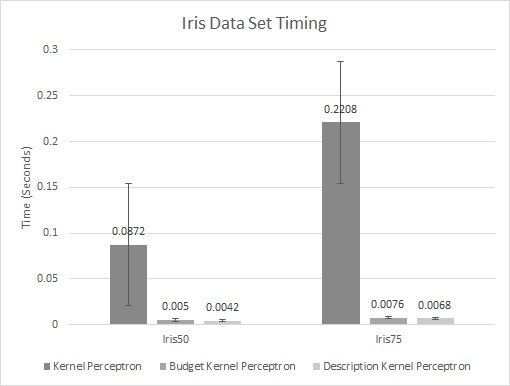
\includegraphics[scale=0.6]{IrisTiming}
 \end{center}
\end{figure}

\begin{table}[h]
 \begin{center}
  \caption{Iris Average Runtimes (Seconds) and Confidence Intervals}
  \label{tab:iristabtiming}
  \begin{tabular}{l|c|c|c|c|c|c}
  \textbf{Trial} & \textbf{KP} & \textbf{95\% CI} & \textbf{Budget KP} & \textbf{95\% CI} & \textbf{Description KP} & \textbf{95\% CI}\\
  \hline
  \textbf{Iris 50/50} & 0.0872 & 0.00342 & 0.005 & 0.00392 & 0.0042 & 0.00431\\
  \textbf{Iris 75/25} & 0.2208 & 0.00563 & 0.0076 & 0.00462 & 0.0068 & 0.00501\\
  \end{tabular}
 \end{center}
\end{table}

\subsection{Sonar Mines vs. Rocks Dataset Performance Results}\label{SonarResults}
The Sonar Mines vs. Rocks Dataset contains 208 examples of 60-dimensional data, representing sonar pings of either underwater explosive mines or roughly cylindrical rocks. This dataset is linearly separable. Like the Iris dataset, the Sonar dataset is not divided into a training set and testing set. Using the same method as the Iris dataset, two Sonar datasets were created with a roughly 50/50 split training and testing (116/92) and a roughly  75/25 split (157/51). The Sonar datasets were further preprocessed by adding a unique integer identifier to the front of each example and changing the labels from M to True and R to False. 
\\The values for each example in the original Sonar dataset are decimals ranging from zero to one. The authors of \cite{MGS17} stated that on the full Sonar dataset, their Perceptron took over 275,000 epochs to converge to a solution. Due to limitations on my machine used for performance experiments, it was not realistic to run my implementations for more than 10,000 epochs. Because of this limitation, the Sonar dataset was normalized from values from zero to one to values between negative one and one to center the examples closer to the zero vector used at the start of training. The normalized data files were used for the generalization error and timing experiments described below. 
\\Again, the generalization error results were found using the RunFile driver for each implementation. All implementations ran for 10,000 epochs. The Budget Kernel Perceptron was limited to 10\% of the training set and the Description Kernel Perceptron to 10\% of the training set as the number of mistakes.
\\The results for the 50/50 split of the Sonar dataset are shown in Table \ref{tab:sonar50gencalc} and for the 75/25 split are in Table \ref{tab:sonar75gencalc}. Only the Kernel Perceptron had results with higher than about 50\% accuracy for both Sonar Datasets. The results for the Budget Kernel Perceptron and Description Kernel Perceptron were disappointing due to the fact that the Sonar datasets violate their underlying assumptions. To produce a model with high accuracy, thousands of misclassifications must be made to incrementally move the hyperplane. Because the dataset contains a maximum of just 208 examples, variants that rely on making a number of mistakes significantly smaller than the number of training examples are bound to have poor performance. The accuracies of the Budget and Description Kernel Perceptron only increase when the number of misclassifications or support vectors is set to the minimum necessary, which means that such a setting will have much worse generalization error compared to the Kernel Perceptron. The Sonar datasets also do not produce nonvacuous bounds due to the size of the training set and the dimensionality of the data.

\begin{table}[p]
 \begin{center}
  \caption{Sonar 50/50 Dataset Observed and Calculated Generalization Error}
  \label{tab:sonar50gencalc}
  \begin{tabular}{l|c|c|c}
  \textbf{ } & \textbf{Kernel Perceptron} & \textbf{Budget KP} & \textbf{Description KP}\\
  \hline
  \textbf{Training Examples} & 116 & 116 & 116\\
  \textbf{Testing Examples} & 92 & 92 & 92\\
  \textbf{Dimensionality} & 60 & 60 & 60\\
  \textbf{Support Vectors} & 116 & 11 & 11\\
  \textbf{Epochs} & 10,000 & 10,000 & 10,000\\
  \hline
  \textbf{Training Accuracy} & 100\% & 55.17\% & 55.17\%\\
  \textbf{Testing Accuracy} & 69.57\% & 51.09\% & 51.09\%\\
  \textbf{Generalization Error} & 30.43\% & 4.08\% & 4.08\%\\
  \hline
  \textbf{eps = 0.001} & 6.66619E+68162 & 1.06487E+6467 & 4.98537E+6370\\
  \textbf{eps = 1} & Would not compute & 1.86671E+6366 & 8.73934E+6269\\
  \end{tabular}
 \end{center}
\end{table}

\begin{table}[p]
 \begin{center}
  \caption{Sonar 75/25 Dataset Observed and Calculated Generalization Error}
  \label{tab:sonar75gencalc}
  \begin{tabular}{l|c|c|c}
  \textbf{ } & \textbf{Kernel Perceptron} & \textbf{Budget KP} & \textbf{Description KP}\\
  \hline
  \textbf{Training Examples} & 157 & 157 & 157\\
  \textbf{Testing Examples} & 51 & 51 & 51\\
  \textbf{Dimensionality} & 60 & 60 & 60\\
  \textbf{Support Vectors} & 157 & 15 & 15\\
  \textbf{Epochs} & 10,000 & 10,000 & 10,000\\
  \hline
  \textbf{Training Accuracy} & 84.08\% & 54.14\% & 54.78\%\\
  \textbf{Testing Accuracy} & 82.35\% & 50.98\% & 50.98\%\\
  \textbf{Generalization Error} & 1.73\% & 3.16\% & 3.8\%\\
  \hline
  \textbf{eps = 0.001} & 7.18546E+92254 & 4.71614E+8818 & 6.48856E+8683\\
  \textbf{eps = 1} & Would not compute & 2.01955E+8682 & 2.77855E+8547\\
  \end{tabular}
 \end{center}
\end{table}

The timing results for the Sonar Datasets are given in Table \ref{tab:sonartabtiming}. These results were found by running 10,000 epochs for each implementation, and the confidence intervals for each implementation are also listed.

\begin{table}[ht]
 \begin{center}
  \caption{Sonar Average Runtimes (Seconds) and Confidence Intervals}
  \label{tab:sonartabtiming}
  \begin{tabular}{l|c|c|c|c|c|c}
  \textbf{Trial} & \textbf{KP} & \textbf{95\% CI} & \textbf{Budget KP} & \textbf{95\% CI} & \textbf{Description KP} & \textbf{95\% CI}\\
  \hline
  \textbf{Sonar 50/50} & 1045.839 & 1.49470 & 79.0278 & 2.06799 & 66.1688 & 1.28507\\
  \textbf{Sonar 75/25} & 2121.471 & 6.43889 & 138.6656 & 4.08308 & 121.6616 & 3.08207\\
  \end{tabular}
 \end{center}
\end{table}

\subsection{Discussion of Generalization Error and Timing Results}\label{ResultsDiscussion}
There are several alternatives to the generalization bound formulation used in the MLCert framework. Mohri and Rostamizadeh \cite{MR13} give the following formulation for their bound, expressed in Equation \ref{MRBound}. For this bound, the authors posit that there are $T$ labeled training examples used to train an on-line algorithm such as the Perceptron, and that these training examples are drawn i.i.d. from the distribution $D$. $L$ represents the loss function used by the algorithm. The authors record the sequence of hypotheses generated by the algorithm as $h_1,...,h_T$. Therefore, the bound aims to minimize the expected error of the algorithm by finding $\hat{h}$. The $\delta$ variable is similar to $eps$ in MLCert's generalization bound. The mathematics behind this bound are based on the average accuracy of each hypothesis in the seqence to find the expected accuracy.

\begin{equation} \label{MRBound}
 E_{(x,y)\sim D}[L(y\hat{h}(x))] \leq \frac{1}{T} \sum_{i=1}^{T} L(y_i h_i(x_i)) + 6\sqrt{\frac{1}{T}\log \frac{2(T+1)}{\delta}} 
\end{equation}

Mohri and Rostamizadeh do not directly give generalization bounds for the Kernel Perceptron, but they do list modifications that can be made to their theorems that account for kernelization. However, this bound requires the storage of the entire sequence of hypotheses through testing. As our system only stores the most recent hypothesis, the MLCert bound cannot look into past hypotheses. Unfortunately, our generalization bounds cannot directly be compared to Mohri and Rostamizadeh's because of this method of formulation.
\\Cesa-Bianchi, Conconi, and Gentile \cite{CBCG04} formalized a generalization bound also based on the sequence of hypothesis created during training. In the authors' bound, where they use risk in place of generalization, the number of training examples is $n$ such that $Z^n$ represents the entire set of training examples. $K$ represents the kernel function used, and the dual kernel, different from the kernel defined in our research as well as by Mohri and Rostamizadeh, is provided in Equation \ref{CBCGKernel}. $\mathcal{M}$ is defined in Equation \ref{CBCGM} as the set of all misclassifications, and $t$ represents the index of a single misclassification. $f$ is the norm of the kernel space. This bound uses hinge-loss instead of the usual zero-one loss function for the Kernel Perceptron, and $\gamma$ defines the margin for the hinge-loss function. The full bound is shown in Equation \ref{CBCGBound}.

\begin{equation}\label{CBCGKernel}
 \sum_{i=1}^{m}\sum_{j=1}^{m} \alpha_i \alpha_j K(x_i, x_j) \geq 0
\end{equation}

\begin{equation}\label{CBCGM}
 \mathcal{M} = {1 \leq t \leq n : H_{t-1}(X_t) \neq Y_t}
\end{equation}

\begin{equation}\label{CBCGBound}
 risk(\hat{H}) \leq \inf_{f\in \mathcal{H}_K:\|f\|\leq1} \inf_{\gamma > 0} \left(D_{\gamma,n}(f, Z^n) + \frac{1}{\gamma n} \sqrt{\sum_{t \in \mathcal{M}} K(X_t, X_t)}\right) + 6\sqrt{\frac{1}{n}\ln \frac{2(n+1)}{\delta}}
\end{equation}

As with the bound by Mohri and Rostamizadeh, Cesa-Bianchi, Conconi, and Gentile define their bound in terms of minimizing $\hat{H}$ from the full set of hypotheses found during training. Again, our generalization bound cannot be directly compared to the above bound because we do not store past hypotheses. Additionally, as our implementations do not use the dual kernel, the kernelization and kernel space described in this paper do not directly correlate to our kernel and parameter spaces.
\\These bounds do, however, show that generalization is an important performance metric, although the exact formulation may vary even for the same or similar algorithms. Our generalization bound calculations are simpler to calculate and rely on fewer variables. 
\\Some trends between datasets and implementations are shown in the generalization and timing analyses. Many of the generalization bounds calculated in this thesis are vacuous. Nonvacuous bounds rely on a very small support set compared to the full training set. Unfortunately, the computer I have had to use for my research is not powerful enough to run experiments with a larger training set size to examine more nonvacuous bounds due to its age and computational capabilities. Vacuous bounds provide no real guarantee for performance, even though the theorems for the generalization bounds have been proved in Coq. Future work to examine the nonvacuous bounds of the Budget and Description Kernel Perceptrons could determine guidelines for the dimensions and size of datasets that will provide nonvacuous bounds.
\\However, the results of the timing analysis, especially for the synthetic datasets, shows that the Budget and Description Kernel Perceptrons are significantly faster to run when the size of the budget or number of mistakes are a fraction of the full size of the dataset. Storing fewer nonessential support vectors saves computation time and resources compared to the Kernel Perceptron.
\\Timing results with the Budget Python implementations also demonstrate that the Haskell implementations have slightly faster run times than Python implementations, even the Python implementation which was optimized using Numpy functions and data structures. While Haskell is not often used for machine learning, it has been demonstrated to be viable for running machine learning algorithms. 
\\The Sonar dataset highlights that the Budget and Description Kernel Perceptrons rely on the either a small number of necessary support vectors or a small number of mistakes compared to the size of the training set. In cases where neither of these assumptions is true, the Budget and Description Kernel Perceptrons will have worse accuracy compared to the Kernel Perceptron. The Kernel Perceptron works best for datasets with a high number of necessary support vectors of many mistakes compared to the size of the training set. Because of this, the Budget and Description Kernel Perceptrons are not always improvements on the performance of the Kernel Perceptron.
\\Finally, the Iris dataset validates that the Kernel Perceptron variants can perform well on a real-world dataset. Because few misclassifications are necessary to produce a hyperplane with perfect accuracy, all variants of the Kernel Perceptron had high performance on the Iris dataset. Overall, these results show that the variants of the Kernel Perceptron can perform well on real and synthetic data.
\section{Chapter Summary}\label{ResultsChapterSummarySection}
These results from the implementations of the Kernel Perceptron, Budget Kernel Perceptron, and Description Kernel Perceptron demonstrate that the generalization error for the Kernel Perceptron can be improved through limiting the size of the support set or placing a limit on the number of mistakes made during training. The conclusions drawn from these results are described in Chapter \ref{ConclusionsChapter}, along with a discussion of future work to be done in the field of machine learning verification.
